\pagestyle{fancy}
\renewcommand{\theUnit}{7}
\ifthenelse{\isundefined{\UnitPageNumbers}}{}{\setcounter{page}{1}}
\rhead{Chapter  \theUnit: Confidence Intervals}
\lhead{Math 3382: Statistical Theory}
%\lhead{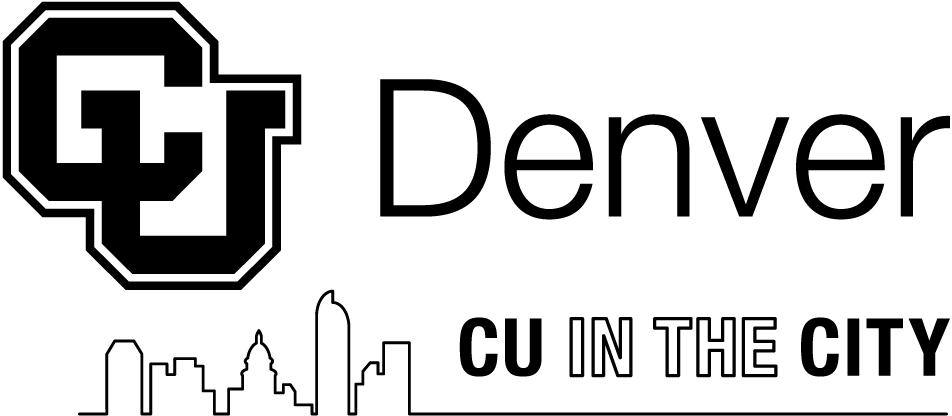
\includegraphics[width=1.25cm]{CUDenver-Logo.png}}
\rfoot{\mypage}
\cfoot{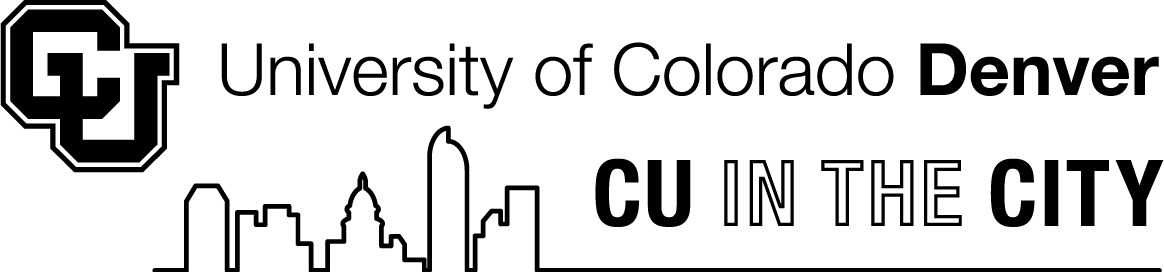
\includegraphics[width=2.25cm]{CUDenver-Logo-coverpage.png}}
\lfoot{Adam Spiegler}
\fancypagestyle{firstfooter}{\footskip = 50pt}
\renewcommand{\footrulewidth}{.4pt}
%%%%%%%%%%%%%%%%%%%%%%%%%%%
\vspace*{-20pt} \thispagestyle{firstfooter}


%\begin{tasks}[counter-format = {(tsk[a])},label-offset = {0.8em},label-format = {\color{black}\bfseries}](2)

\pagebegin{Section 7.1: Confidence Intervals for Means}

\begin{multicols}{2}
What is the average sea surface temperature (SST) on Earth? There are a variety of methods that have been used to estimate this parameter. One possible method would be to randomly select locations and times around the world from which to sample, and then compute the average temperature of the sample.

\columnbreak

\begin{center}
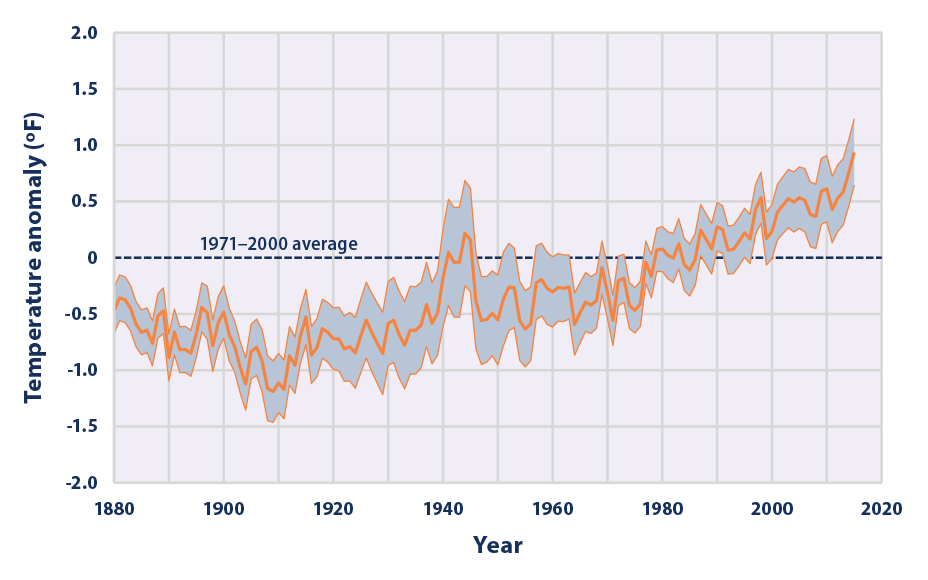
\includegraphics[width=0.48\tw]{16/fig-sea-surface.png}
\end{center}

Image Credit: United States Environmental Protection Agency\footnote{\href{https://www.epa.gov/climate-indicators/climate-change-indicators-sea-surface-temperature}{\underline{https://www.epa.gov/climate-indicators/climate-change-indicators-sea-surface-temperature}}, Accessed Nov. 1, 1019.}
\end{multicols}

\bi
\ii We have already seen that one unbiased estimator for the parameter $\mu$ is the sample mean $\bar{x}$.
\ii However, based on one sample we have no idea how far off $\bar{x}$ is from the actual value of $\mu$.
\ii One way build some uncertainty into the estimate is to use a bootstrap distribution to get a range of plausible values.
\ii In chapter 7, we will learn some other methods for constructing confidence intervals.
\ei

\bb
\ii Let's imagine instead of the sea surface, or population $X$ is all of the lyrics to Prince's song ``Raspberry Beret''. Like the sea surface, imagine the population $X$ consists of so many words that it is impractical to calculate the mean length of all words in ``Raspberry Beret''.  We will measure the length of a word by the number of letters in the word.
\bb
\ii True or false: The values of the $\bar{X}$'s will be different for different random samples. \bs
\ii True or false: The value of $\mu$ will be different for different random samples. \bs
\ii Prove that $P\left( \bar{X} - 1.96 \cdot \sigma_{\bar{X}} < \mu < \bar{X}+1.96 \cdot \sigma_{\bar{X}} \right) = 0.95$. \vfill
\ii Explain what $P\left( \bar{X} - 1.96\cdot  \sigma_{\bar{X}} < \mu < \bar{X}+1.96 \cdot \sigma_{\bar{X}} \right) = 0.95$ means in words. \vfill
\ee

\clearpage

\ii Open the file \textit{Raspberry Beret.R}.  Let's assume for now that although we do not know the value of the parameter $\mu$ (average number of letters of all words in the song), we do know that $\sigma^2 = 3.45$ letters.
\bb
\ii Using the sample function, pick a random sample of 30 words (without replacement) from all the lyrics. What are the 30 randomly selected words in your sample? \vspace{1.25in}
\ii Calculate the mean number of letters in each word in your sample and make a histogram of the length of the words in your sample. \vspace{0.5in}
\ii Using the CLT what is the value of $\sigma_{\bar{X}}$, the standard error of the sampling distribution for $\bar{X}$? \vspace{1in}
\ii Based on your previous answers, give an interval of values that has a 95\% chance of containing the actual value of $\mu$. \vfill
\ee
\ee

\bbox
For a sample size $n$ drawn from a normal distribution with unknown $\mu$ and known $\sigma^2$, a 95\% confidence interval for the mean is
%\[ \bar{X} - 1.96 \frac{\sigma}{\sqrt{n}} < \mu <  \bar{X} + 1.96 \frac{\sigma}{\sqrt{n}}.\]
\vspace{1in}

If we draw 1000's of random samples size $n$ from a normal distribution with parameters $\mu$ and $\sigma$ and compute a 95\% confidence interval from each sample, then about 95\% of the intervals would contain $\mu$.
\ebox

\clearpage
\pagebegin{Interpreting Confidence Intervals}

\bb[resume]
\ii A researcher calculates collects a random sample of words and gets a 95\% confidence interval for the mean length of a word that is from $2.57$ letters to $3.90$ letters. For each statement, determine whether the interpretation is correct or not. If not, explain why not.
\bb
\ii There is a 95\% chance that randomly selected word has between $2.57$ and $3.90$ letters. \vfill
\ii There is a 95\% chance that the mean length of all words in ``Raspberry Beret''  is between $2.57$ and $3.90$ letters. \vfill
\ii The interval from $2.57$ and $3.90$ letters will contain the mean length of all words in ``Raspberry Beret''  95\% of the time. \vfill
\ii 95\% of all random samples of size $n=30$ words have a sample mean length between $2.57$ and $3.90$ letters. \vfill
\ii We are 95\% confident that the mean length of all words is between $2.57$ and $3.90$ letters. \vfill
\ee

\ii What are some cautions to keep in mind when interpreting confidence intervals? \vfill

\clearpage

\pagebegin{Changing the Confidence Level}

\ii Researchers want to estimate the average length of all female Kamodo dragons. The pick a random sample of female Kamodo dragons with the following weights (in pound):
\[ 145, 178, 142, 139, 160, 190, 168, 122; \]
and suppose they know that $\sigma = 25$ pounds.
\bb
\ii Give a 95\% confidence interval, and interpret the meaning of your answer. \vfill
\ii Give a 90\% confidence interval, and interpret the meaning of your answer. \vfill
\ii As we decrease the \textbf{confidence level} of the interval, what happens to the width of the interval estimate? \vfill
\ee
\ee

\bbox
If $X_i \sim N(\mu, \sigma^2)$, $i=1,2,\ldots , n$ with known $\sigma$, and confidence level equal to CL, then a corresponding
confidence interval is given by
\[  \bar{X} - z_{\alpha/2} \cdot \frac{\sigma}{\sqrt{n}} < \mu < \bar{X} + z_{\alpha/2} \cdot \frac{\sigma}{\sqrt{n}}, \]
where the area under $N(0,1)$ between $\pm z_{\alpha/2}$ is equal to the confidence level.

The distance $\mbox{ME} = z_{\alpha/2} \cdot \frac{\sigma}{\sqrt{n}}$ is called the \colorb{\textbf{Margin of Error (MOE)}} of the
confidence interval.
\ebox

\clearpage

\pagebegin{Section 7.1: Confidence Intervals for Means, $\sigma$ Unknown}

In most real-life settings, we do not know $\mu$ or $\sigma$. In deriving a confidence interval, we have used $\bar{X}$ as an estimate of $\mu$, so it seems natural to use the sample standard deviation $S$ as an estimate for $\sigma$. The plot on the left gives a histogram for the standardized sampling distribution  $Z' = \frac{\bar{X}-\mu}{s/\sqrt{n}}$ and the plot on the right is a qqplot comparing $Z'$ to $N(0,1)$.  

\begin{center}
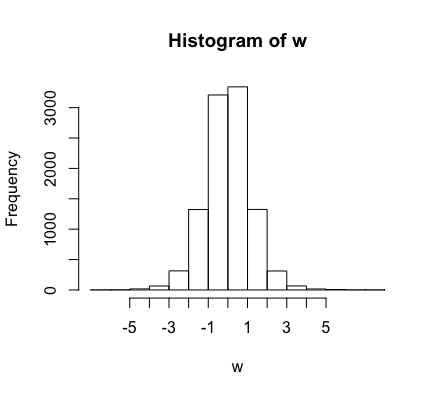
\includegraphics[width=0.3\tw]{16/fig-stand-samp.png} \ \ \ \ \ \ \ \ \
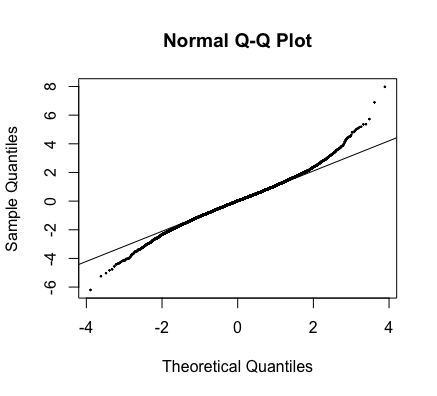
\includegraphics[width=0.3\tw]{16/fig-qq-samp.png}
\end{center}

\bbox
\textbf{T Confidence Interval for a Normal Mean With Unknown $\mathbf{\sigma}$:} If $X_i \sim N(\mu, \sigma^2)$, $i=1,2,\ldots , n$ with unknown $\sigma$, and confidence level equal to CL, then a corresponding confidence interval is given by
\[  \bar{X} - t_{\alpha/2} \cdot \frac{s}{\sqrt{n}} < \mu < \bar{X} + t_{\alpha/2} \cdot \frac{s}{\sqrt{n}}, \]
where the area under the $t$-distribution with $n-1$ degrees of freedom between $\pm t_{\alpha/2}$ is equal to the confidence level.
\bi
\ii The command \colorb{\textbf{qt($0.975$, \ $7$)}} gives the $0.975$ quantile from a $t$-distribution with 7 degrees of freedom.
\ii The command \colorb{\textbf{ pt($2.5$, \ $7$)}} gives the $P(T < 2.5)$ for random variable $T$ from a $t$-distribution with 7 degrees of freedom
.
\ii Use a $t$-distribution table to estimate areas under $t$-distributions.
\ii The command \colorb{\textbf{t.test(samp\_name, conf.level = 0.95)$\$$conf}} will give a 95\% confidence level.
\ei
\ebox

\begin{multicols}{2}
\begin{center}
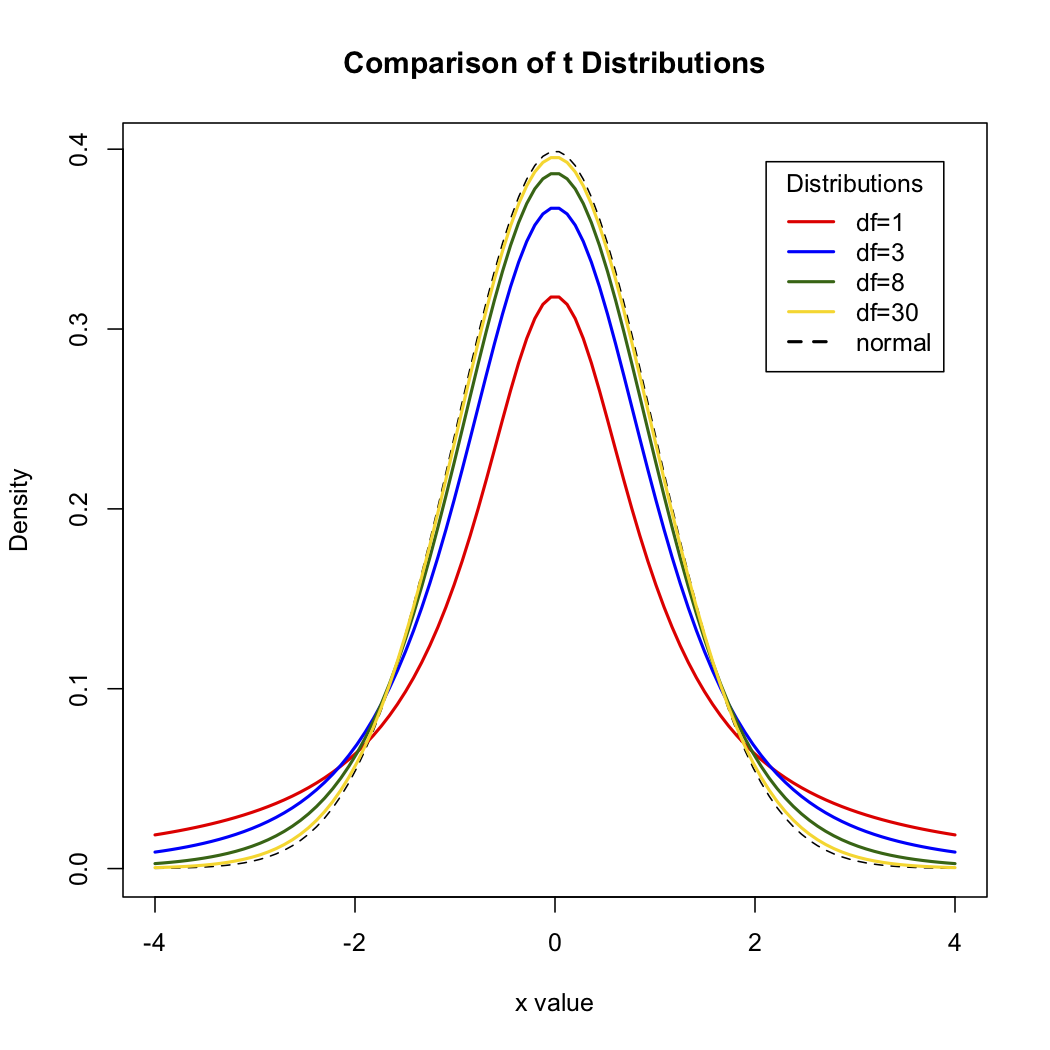
\includegraphics[width=0.33\tw]{16/fig-tdist.png}
\end{center}
\columnbreak

\bbox
\bi
\ii If the underlying population is known to be symmetric (but not necessarily  normal), then a $t$-distribution with $n-1$ degrees of freedom is still a good estimate.
\ii The more skewed the population is, the less accurate using a $t$-distribution becomes.
\ei
\ebox
\end{multicols}

\clearpage
\pagebegin{Practice}

\bb[resume]
\ii Using the dataset \textit{NCBirths2004}, give a 99\% confidence interval for the mean weight (in grams) of all babies born in North Carolina in 2004. Interpret the meaning of your answer in practical terms. Show your work and code used. 
\ee

\vfill

\pagebegin{Section 7.1: Confidence Intervals for a Difference in Means}

\bb[resume]
\ii Let $X$ and $Y$ be independent random variables with $X \sim N(\mu_1, \sigma_1^2)$ and $Y \sim N(\mu_2, \sigma_2^2)$. Using properties of expected value and variance, show for sample sizes $n_1$ and $n_2$, respectively, that
\[ \Exp(\bar{X}-\bar{Y}) = \mu_1-\mu_2 \ \ \ \mbox{and} \ \ \ \Var(\bar{X}-\bar{Y}) = \frac{\sigma_1^2}{n_1} +  \frac{\sigma_2^2}{n_2}.\]
\ee

\vfill

\bbox
\textbf{T Confidence Interval for a Difference in Means:} If $X_i \sim N(\mu_1, \sigma_1^2)$, $i=1,2,\ldots , n_1$ and $Y_j \sim N(\mu_2, \sigma_2^2)$, $j=1,2,\ldots , n_2$, then an approximate confidence interval for $\mu_1 - \mu_2$ is given by
\[ (\bar{X} - \bar{Y}) \pm  t_{\alpha/2} \cdot  \sqrt{\frac{S_1^2}{n_1} +  \frac{S_2^2}{n_2}}\]
where the area under the $t$-distribution with $df$ degrees of freedom between $\pm t_{\alpha/2}$ is equal to the confidence level.
\bi
\ii Informally, we can use the smaller of $n_1-1$ and $n_2-1$ as the degrees of freedom.
\ii A more accurate rule is Welch's approximation:
\[ v = \frac{\left( s_1^2/n_1+ s_2^2/n_2 \right)^2}{ \frac{(s_1^2/n_1)^2}{n_1-1} + \frac{(s_2^2/n_2)^2}{n_2-1}}.\]
\ii If the confidence interval for a difference in means contains $0$, then it is plausible that there is no difference in the two means.
\ii The command \colorb{\textbf{t.test(samp1\_name, samp2\_name, conf.level = 0.95)$\$$conf}} will give a 95\% confidence level for the difference in means.
\ei
\ebox

\pagebegin{Practice}

\bb[resume]
\ii A study randomly assigned students to take notes either writing them by hand or using a laptop. The resulting scores of the students on a test of the material are summarized in the table below:
\begin{center}
\begin{tabular}{lccc}
\hline
Group & $n$ & $\bar{x}$ & $s$ \\
\hline
By hand & 38 & $25.6$ & $10.8$\\
Laptop & 40 & $18.3$ & $9.0$\\
\end{tabular}
\end{center}
\bb
\ii Give a 95\% confidence interval using an approximation with a $t$-distribution with degrees of freedom equal to the $n_{\rm min} -1$. \vfill
\ii Interpret the meaning of your answer. Do you believe there is a difference in the exam scores of the two groups? Explain. \vspace{1.5in}
\ii If you use Welch's approximation, you get $v = 72.1368 \approx 72$. Give a 95\% confidence interval using an approximation with a $t$-distribution with degrees of freedom equal to the $v=72$. \vfill
\ee 

\ee
